\documentclass[twocolumn]{article}\usepackage[]{graphicx}\usepackage[]{xcolor}
% maxwidth is the original width if it is less than linewidth
% otherwise use linewidth (to make sure the graphics do not exceed the margin)
\makeatletter
\def\maxwidth{ %
  \ifdim\Gin@nat@width>\linewidth
    \linewidth
  \else
    \Gin@nat@width
  \fi
}
\makeatother

\definecolor{fgcolor}{rgb}{0.345, 0.345, 0.345}
\newcommand{\hlnum}[1]{\textcolor[rgb]{0.686,0.059,0.569}{#1}}%
\newcommand{\hlstr}[1]{\textcolor[rgb]{0.192,0.494,0.8}{#1}}%
\newcommand{\hlcom}[1]{\textcolor[rgb]{0.678,0.584,0.686}{\textit{#1}}}%
\newcommand{\hlopt}[1]{\textcolor[rgb]{0,0,0}{#1}}%
\newcommand{\hlstd}[1]{\textcolor[rgb]{0.345,0.345,0.345}{#1}}%
\newcommand{\hlkwa}[1]{\textcolor[rgb]{0.161,0.373,0.58}{\textbf{#1}}}%
\newcommand{\hlkwb}[1]{\textcolor[rgb]{0.69,0.353,0.396}{#1}}%
\newcommand{\hlkwc}[1]{\textcolor[rgb]{0.333,0.667,0.333}{#1}}%
\newcommand{\hlkwd}[1]{\textcolor[rgb]{0.737,0.353,0.396}{\textbf{#1}}}%
\let\hlipl\hlkwb

\usepackage{framed}
\makeatletter
\newenvironment{kframe}{%
 \def\at@end@of@kframe{}%
 \ifinner\ifhmode%
  \def\at@end@of@kframe{\end{minipage}}%
  \begin{minipage}{\columnwidth}%
 \fi\fi%
 \def\FrameCommand##1{\hskip\@totalleftmargin \hskip-\fboxsep
 \colorbox{shadecolor}{##1}\hskip-\fboxsep
     % There is no \\@totalrightmargin, so:
     \hskip-\linewidth \hskip-\@totalleftmargin \hskip\columnwidth}%
 \MakeFramed {\advance\hsize-\width
   \@totalleftmargin\z@ \linewidth\hsize
   \@setminipage}}%
 {\par\unskip\endMakeFramed%
 \at@end@of@kframe}
\makeatother

\definecolor{shadecolor}{rgb}{.97, .97, .97}
\definecolor{messagecolor}{rgb}{0, 0, 0}
\definecolor{warningcolor}{rgb}{1, 0, 1}
\definecolor{errorcolor}{rgb}{1, 0, 0}
\newenvironment{knitrout}{}{} % an empty environment to be redefined in TeX

\usepackage{alltt}
%\documentclass[10pt]{article}
\usepackage{color}
\usepackage[italian,english]{babel}
\usepackage[colorlinks,bookmarksopen,bookmarksnumbered,citecolor=red,urlcolor=red]{hyperref}
\usepackage[margin=2cm]{geometry}
\usepackage{bm}
\usepackage{tikz}
\usepackage[utf8x]{inputenc}
\usepackage{amsmath,amssymb}
\usepackage{caption}
\captionsetup{font=footnotesize}
\usepackage{apacite}
% \usepackage[bottom]{footmisc} 

%\newcommand\BibTeX{{\rmfamily B\kern-.05em \textsc{i\kern-.025em b}\kern-.08em
%T\kern-.1667em\lower.7ex\hbox{E}\kern-.125emX}}

\usepackage{float}
\floatstyle{boxed}
\newfloat{program}{btp}{lop}
\floatname{program}{Box}
\usepackage{mdframed}
\definecolor{boxcol}{RGB}{213,226,238}
\newmdenv[linecolor=boxcol,backgroundcolor=boxcol]{comments}




\IfFileExists{upquote.sty}{\usepackage{upquote}}{}
\begin{document}

\title{\textbf{\textit{How do my distributions differ?} \\ Significance testing for the Overlapping Index \\ using Permutation Test}} %%%%% Overlapping test: Significance testing for the Overlapping Index \\ using Permutation Test
\author{Ambra Perugini $^1$, Giulia Calignano $^1$, Massimo Nucci $^2$, Livio Finos $^3$, Massimiliano Pastore $^1$}

\maketitle



\begin{abstract}
The present contribution aims to introduce the application of the permutation test to the Overlapping Index to estimate effects of interest in psychological science. Starting with most common scenarios in psychological sciences the paper highlights the importance of relying on statistical methods that are resilient to the complexities inherent in psychological data, where assumption violations are often inevitable. Subsequently, we present a Simulation study to illustrate the practical implications and reliability of the proposed test in comparison to most commonly used tests. The findings show the good control of Type I error of the $\zeta$ overlapping test and how this approach outperforms in terms of power all other tests considered in the simulation, already prom small samples. The paper provides practical guidance and demonstrates the advantages of this methodology, emphasizing its potential to enhance transparency and rigor in psychological data analysis by shifting focus from traditional significance testing to comprehensive distributional evaluations.
\end{abstract}

\section{Statistical testing choices in Psychology}

    Methodological choices in cognitive and behavioral sciences aim to combine data richness with data collection feasibility, and at the same time they aim to land on valid interpretation based on reliable and robust statistical methods. Classic examples, like reaction times, demonstrate how specific measures have achieved such an acceptable trade-off, and for example, this is true even by comparing the framework of in lab \textit{vs} online data collection \cite{semmelmann2017online}. Nevertheless, even in the fortunate case of reaction times which have widespread and solid epistemic rationale of use \cite{grosjean2001timing, proctor2018hick, silverman2010simple} significance testing often relies on the rigid application of a few statistical methods that have gained popularity among the scientific community and are perpetrated \textit{perinde ac cadaver} by formal guidelines \cite{cumming2012statistical}, even if their limits and risks have always been noted in the field of psychology and beyond \cite{boneau1960effects}. 
    

   In fact, there is a growing caution against blindly using statistical tools and analytical methods without a deep understanding of their assumptions and implications \cite{scheel2021hypothesis}. In other words, it is increasingly apparent that relying solely on significance testing as a trustworthy measure is improbable without considering the assumptions inherent to specific statistical methods, such as the t-test, across various scenarios in psychology. In fact, considering the particular circumstances of application has consistently been crucial advice when deciding on significance testing methods \cite{fisher1925theory}. 
   
   %%% H0 è la differenza tra le distribuzioni, sputtanare t-test. H0 vale solo nel prio riquadro [1] in fig 4. scenario dove tutti giocano secondo la loro h0 e secondo scenario dove h0 è che le dist sono uguali, poi sbaglierebbero tutti tranne il nostro. Mettere grafico 6 nei supplementari ed essere aggressivi mostrando che il nostro va meglio di tutti con h0 = dist uguali. 
   %%%% c'erano sim aggiuntive con due dist non normali le mettiamo??
   %%%% valore aggiunto, controlli tutto con un solo test.
   %%%% pompare nei risultati che già con 70 soggetti il perm test ha 80% di potenza
   %%% a cosa sei interessato? se vengono dalla stessa popolazione o se sono diverse, poi uno va a vedere come sono diverse. scenario 1 contro tutti gli altri.
   %%%% levare i 4 scenari
   %%%% Poi implementare nel pacchetto descrittive delle due distribuzioni
   %%%% aggiungiamo descrittive in fig 2 (test sul dataset reale)
   %%%% fig 6 invece di probability of false positive, power of detecting true positive effects
   %%%% Oltre che uguale varianza assume normalità l'F test. Aggiungere i vari assunti. Nella discussion: a volte guardiamo se le varianze vanno bene ma violiamo assunti di normalità. Funziona comunque il t test grazie al teorema del limite centrale. 
    
    \vspace{0.2cm}
    
   The present contribution aims to present a novel approach for statistical testing, in particular for comparing two groups/conditions. Specifically, the present work proposes applying the Permutation test \cite{pesarin2001} alongside the Overlapping index  \cite< $\eta$,>{pastore2019measuring} to compare empirical distributions. 
Importantly, by simulating different scenarios, we compare widely used statistical tests in Psychological Sciences with this novel approach to evaluate the performance in controlling type I error and power. Understanding and applying significance testing properly is crucial to deriving meaningful conclusions from psychological research. Accordingly, we offer an alternative tool to manage the assumptions underlying these analytical approaches, and increase awareness in significance testing in psychology. But above all, and even most importantly, the advantage of the Overlapping Index and its test is to take into account at the same time mean, variance and shape with a single test.

\vspace{0.2cm}
 Considering that parametric tests, such as linear models, used for statistical inference require strong assumptions that are unlikely to be respected in the aforesaid field, such as normality and homoscedasticity, alternative methods become optimal. The use of non-parametric methods is particularly beneficial when these assumptions are violated \cite{AAAA}. Specifically, when using a t-test to compare two groups or two experimental conditions using a given variable, it functions as a straightforward version of linear regression. This statistical process necessitates assumptions about the error terms, such as their independence and normal distribution, to be met. In cases such as reaction times, these assumptions might be violated if they are not properly addressed. Most importantly, two populations might present the same mean, yet their distributions largely differ in other characteristics, such as variability, leading to genuinely distinct groups (see figure \ref{fig:equalmeans}). 

\vspace{0.2cm}
The remainder of this article is structured as follows. First, we introduce the concept of the Overlapping Index, providing foundational definitions and highlighting its importance. Next, we define the Permutation approach and explore its application to the Overlapping Index, showcasing its relevance in statistical analysis. Subsequently, we present a Simulation study to illustrate the practical implications and trustworthiness of the overlapping index utilizing permutations.
% We do so by comparing several statistical tests: the t-test for independent samples assuming equal variance, the Welch test for independent samples, the Wilcoxon test for independent samples, the Permutation test on the Overlapping index, which serves as a measure of intergroup differences, the F test for homogeneity of variances, and the Kolmogorov-Smirnov test for comparing two distributions. 

The rationale behind these steps involves first introducing the concept of the Overlapping Index ($\eta$), which is crucial because it provides an intuitive measure of similarity between distributions by quantifying the overlapping area of their empirical density functions, a common question in quantitative psychology. The Permutation approach is then defined and applied to the Overlapping Index, demonstrating how nonparametric methods can offer insights without relying on typical parametric assumptions. Specifically, the Permutation test involves shuffling data points to generate a sampling distribution, allowing the calculation of a $p$-value and highlighting its utility in assessing the statistical significance when comparing two groups/conditions. Next, the Simulation study uses a set of different combinations of parameters to simulate various scenarios that might meet or violate the assumptions of different statistical tests, modeling a range of conditions reflective of real-world complexities in psychological research. This simulation facilitates the evaluation of the statistical power (probability of correctly rejecting a false null hypothesis) and the type I error rate (likelihood of incorrectly rejecting a true null hypothesis) of each approach. To this end, several statistical tests are compared: the t-test for independent samples, assuming equal variances; the Welch test, which does not assume equal variances; the Wilcoxon test, suitable for ordinal data or when normality is not assumed; the Permutation Test on the Overlapping Index, providing a non-parametric approach to evaluate distributional differences; the F test for examining the homogeneity of variances; and the Kolmogorov-Smirnov test for comparing two distributions regardless of their underlying forms. These results enable researchers to visualize and comprehend the reliability and utility of each approach, particularly valuable in scenarios commonly encountered in quantitative psychology, where navigating data characteristics and adhering to or deviating from test assumptions is crucial.

Finally, we discuss the results, offering insights into the strengths and limitations of the Permutation-based Overlapping index and its potential applications in psychological sciences.


\section{Overlapping Index}

% Cognitive and experimental researchers regularly strive to uncover evidence that supports their hypotheses by examining statistical differences or similarities among groups or conditions. Frequently, this involves measuring the difference between two distribution within the same dependent variable, basically relying on their mean values using metrics like the t statistic, Cohen's \textit{d}, or \textit{U} statistics. The goal in each scenario is to estimate the magnitude of these differences to identify them as significant effects. However, a complementary perspective can be gained through the overlapping index ($\eta$), which intuitively quantifies the common area between two or more probability density functions. This measure serves as an additional tool for comparing distributions, where greater overlap indicates similarity, and a decrease in $\eta$ signals divergence \cite{pastore2019measuring}.

\vspace{0.2cm}
The overlapping index ($\eta$) is an intuitive way to define the area intesected by two or more empirical density functions \cite{pastore2019measuring}. In a simple way, two distributions are similar when their distribution functions overlap, and as $\eta$ diminishes, the two distributions differ.
The $\eta$ index varies from zero -- when the distributions are completely disjoint -- and one -- when they are completely overlapped \cite{pastore2018overlapping}. The simple interpretation of the overlapping index ($\eta$) makes its use particularly suitable for many applications \cite<e.g.>{sirbiladze+al:2024,habibi+al:2024,ricote+al:2024,rossi+al:2024,einbeck+al:2024,wachendorfer+oeberst:2024,rohrbach:2024,hawkins+al:2024,upadhayay+al:2024,conversano+al:2024,pietrabissa+al:2024,nougaret+al:2024,greene+al:2024,schuetze+yan:2023,karrobi+al:2023,garofalo+al:2022,jensen+sanner:2021}. %aggiungere tante cit

More formally, assuming two probability density functions $f_A (x)$ and $f_B (x)$, the overlapping index $\eta: \mathbb{R}^n \times \mathbb{R}^n \to [0,1] $ is formally defined in the following way:


\begin{eqnarray}
\eta (A,B) = \int_{\mathbb{R}^n} min [f_A (x),f_B (x)] dx
\end{eqnarray} 

where, in the discrete case, the integer can be replaced by summation. As previously mentioned, $\eta (A,B)$ is normalized to one and when the distributions of A and B do not have points in common, meaning that $f_A (x)$ and $f_B (x)$ are disjoint, $\eta (A,B) = 0$. This index provides an intuitive way to quantify the agreement between $A$ and $B$ based on their density functions \cite{inman1989overlapping}. 



%%%% aumentare n

\vspace{.3cm}

To quickly illustrate an example of the overlapping area in figure \ref{fig:equalmeans} are represented two different empirical densities. In panel [A], are depicted two density distributions, a Normal(10,2) and a Uniform(0,20); note that the two distributions have the same mean (10), but different variance, 4 and 33.3 respectively. % mettiamo anche il vero valore di overlapping?
In the panel [B] are represented the empirical densities of two random samples of 30 observations drawn from the two populations specified as in panel [A]; the estimated overlapping area being $\eta = 0.46$.

\vspace{.3cm}

% The true $\eta = round( integrate( min_normal_uniform, -Inf, Inf, normPars = normPars, unifPars = unifPars )$value, 2) $.

The figure \ref{fig:equalmeans} shows how two distributions with almost same mean could still be very different from each other with the overlapping area being $\hat{\eta} = 0.46$. In this case, the t-test focuses on mean differences, therefore correctly does not rejects the null hypothesis, even though the degree of similarity of the two densities is only 46\%, in other words, the difference is about 54\%. Moreover, we remind that the t-test in this case is far from ideal as the two distributions have different variances.




\begin{knitrout}
\definecolor{shadecolor}{rgb}{0.969, 0.969, 0.969}\color{fgcolor}\begin{figure}

{\centering 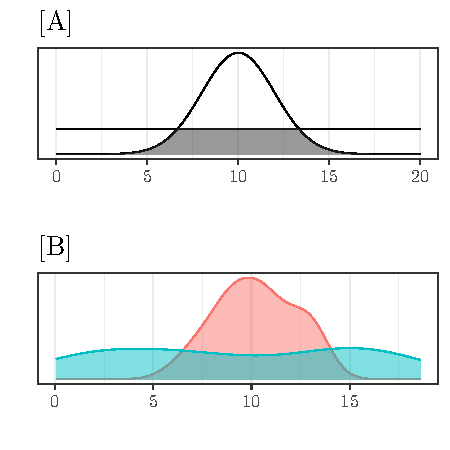
\includegraphics[width=\maxwidth]{figure/equalmeans-1} 

}

\caption[Comparison of a normal distribution and a uniform distribution with same mean, 10, and different variances, 4 and 33.3, respectively]{Comparison of a normal distribution and a uniform distribution with same mean, 10, and different variances, 4 and 33.3, respectively.}\label{fig:equalmeans}
\end{figure}

\end{knitrout}


%In this case, a t-test would not be able to detect such difference, as it does not take into account the different variance in the two groups. Even when using a Welch test, which does not assume equal variance, the test does is less informative ($t = TTESTUNEQUAL$statistic$, $p = TTESTUNEQUAL$p.value$) compared to the overlapping index.



\subsection{Permutation approach}

Permutation tests, also known as randomization tests, are a class of nonparametric statistical significance tests. The concept dates back to the work of R.A. Fisher in the 1930s, in particular his book "The Design of Experiments" \cite{fisher:1935}. The theoretical foundations were further developed by E.J.G. Pitman in his seminal papers of 1937 \cite{pitman1937significance} and 1938 \cite{pitman1938significance}. The basic principle of permutation testing is based on the idea of rearranging observed data to generate a null distribution. This approach assumes that if the null hypothesis is true, then all possible arrangements of the data are equally likely, i.e., each permuted sample has the same probability as the observed one. By resampling the data, we can obtain the distribution of the test statistic under the null hypothesis without making any assumptions about the underlying data generating process. This is particularly valuable when dealing with small sample sizes or when the assumptions of parametric tests are not met. The observed test statistic is then compared to this empirically derived null distribution to determine the probability of obtaining such a result by chance alone \cite{pesarin2001}.
The permutation approach allows for the adoption of any test statistic chosen by the user.
For example, if we are thinking about comparing the means of the two samples, we could choose a $t$-test statistic; the data in the two groups are permutated and the $t$ value is calculated each time. If the two groups come from the same population, the $t$-statistic computed on the observed data should be close to 0; the $t$-statistic computed on randomly permuted data will also give values close to zero. Therefore, the randomly generated test statistic and the observed one have the same -- nonparametric -- distribution.  Otherwise, if
the two groups come from populations with different means, the $t$-statistic computed on the observed data will be far from zero, while the $t$-statistic computed on the permuted data will be around zero.

The $p$-value is the probability of obtaining an equal or more extreme $t$-statistic compared to the observed one.
observed:
\begin{eqnarray}
p=\frac{(\#_{b=1}^B |t_b|\geq |t|)+1}{B+1}
\end{eqnarray}

where $B$ is the number of random permutations, $t$ is the $t$-statistic computed on the observed data, $t_b$ are those computed on the permuted data.

The test will have power -- i.e., the probability of getting a $p\leq \alpha$ when the two samples are really different -- very close to the parametric $t$-test, and it will retain control over false positives even when the assumptions of normality are not met.

It is important to note that the choice of which $t$-statistic to use is a user choice; different test statistics (e.g., difference of mean ranks, Kolmogorov-Smirnov, etc.) will produce tests with different power. For example, if the two samples differ only in their variability and not in their mean, the permutation test based on the $t$-statistic will have little or no power to detect that the two samples come from different populations.
In this direction, this paper proposes to use the overlap index as a test statistic that results to be powerful under a wide range of difference in distributions.

{\bf Remark 1} The choice to add a $+1$ in the numerator and denominator is a choice supported by many authors \cite{phipson2010permutation,hemerik2018exact} and ensures that the probability of false positives is less than or equal to $\alpha$.

{\bf Remark 2} As one can understand, the $p$-value may change depending on the permutations that are drawn. By increasing the number of permutations $B$, the results will change less and less. Since the number of possible permutations is finite, it is preferable, if possible, to explore the set of them (i.e., to compute the statistics on all possible permutations of the data). This set of all possible rearrangements of the data is, in fact, the orbit of the sample that allows us to compute the exact $p$-value - i.e., the exact probability of observing a test statistic that is as extreme or more extreme than that observed in the data. In this case, $B=\binom{n}{n_1} = \frac{n!}{n_1!(n-n_1)!}$ and the $p$-value formula reduces to $$p=\frac{(\#_{b=1}^B |t_b|\geq |t|)}{B}$$ since the test statistic computed on the observed data is certainly in this set.


\subsection{Application of permutation test to the overlapping index}

Even though the overlapping index has a simple interpretation, one could argue that it does not provide information on the significance of $\eta$, therefore, we decided to implement permutation testing to offer to the ones interested a value of significance. In particular, we implemented permutations test, to give a tool that tests differences in distributions without assumptions, offering a valid alternative in cases in which traditional assumtions are not met. 

% in cases where other tests' assumptions would be violated.

If we are reasoning from the perspective of Null Hypothesis Significance Testing (NHST), we should define the null hypothesis as follows: $H_0: \eta = 1$,  meaning that there is complete overlap between the theoretical densities in the two populations from which we sample the data. For this reason, it is more intuitive to work with the complement of $\eta$, which is  $1-\eta = \zeta$ which is the area of non-overlap, therefore, defining the null hypothesis as  $H_0:\zeta = 0$, once again meaning that there is no difference between the densities of the two populations. Obviously, this does not change the results, but only the way in which they are interpreted. When testing the difference between the two distributions, we will no longer be working with $\eta$, but with the complement $\zeta$. 








\begin{knitrout}
\definecolor{shadecolor}{rgb}{0.969, 0.969, 0.969}\color{fgcolor}\begin{figure}[!t]

{\centering 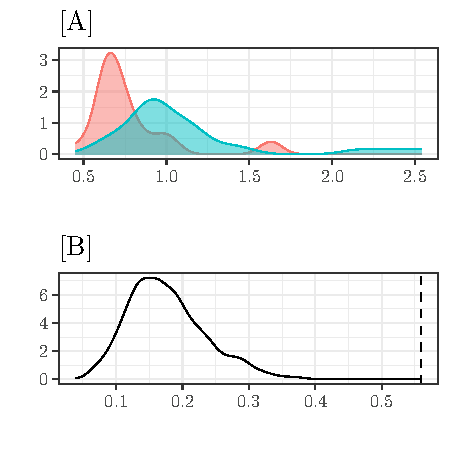
\includegraphics[width=\maxwidth]{figure/ex2-1} 

}

\caption{[A] Distribution of reaction times of word reading of high and low frequency words in English, in this case the non-overlapping area is $\hat{\zeta} = 0.56$; [B] Distribution of $\hat{\zeta}$ obtained with 2000 permutations of the data.}\label{fig:ex2}
\end{figure}

\end{knitrout}

The algorithm estimates the value of $\zeta$ on the observed data ($\hat{\zeta}$). Then, through permutation, the observed values of the two groups are randomly re-assigned to the groups for B times, estimating again the new value of  $\hat{\zeta}_b$. The times in which the estimate of $\hat{\zeta}_b$ on permuted data is higher or equal than the one observed on real data is estimated ($\hat{\zeta}_b \geq \hat{\zeta}$) and then the found value is divided by B, returning the $p$-value. 
A typical example of data not respecting previously said assumptions is reaction times and for this purpose we present a real case of a dataset available online \cite{Oksuz_Rebuschat_2024} on reaction times of word reading of high and low frequency words in English and we implement on the overlapping function the permutation test. 

In the figure \ref{fig:ex2}[A] are represented the densities of reaction times of word reading of high and low frequency words in English from a sample of two groups of 30 observations each; the two distributions have mean 0.78 and 1.11, variance 0.07 and 0.22, and skewness 2.32 and 2.02 respectively. The obtained value of $\hat{\eta}$ is 0.44, and consequently $\hat{\zeta}$ is 0.56. In figure \ref{fig:ex2}[B] is represented the distribution of the values of $\hat{\zeta}$ obtained with 2000 permutations; we can calculate the $p$-\emph{value} as follows:

\begin{eqnarray*}
p = \frac{(\# \hat{\zeta}_b \geq \hat{\zeta})+1 }{B+1} = \frac{1}{ 2001 } %= \ensuremath{4.998\times 10^{-4}}
\end{eqnarray*}

Given that $p < .001$, we can conclude that the difference is statistically significant; in this case the $t$ test give the same conclusion $t_{(58)} = 3.34$, $p = .001$, but we remind that the $t$-test evaluates only the difference between the means and requires assumtions that in this scenario are clearly not met.

\subsection{Practical application}

The overlapping test is easily performed using the \texttt{overlapping} R package  \cite{overlapping:package}. In the following, we briefly present a simple example.  




First, we simulate two different samples, each with $n = 50$: one from a Normal(3,2) distribution and another from a $\chi^2(3)$ distributions:
\begin{knitrout}
\definecolor{shadecolor}{rgb}{0.969, 0.969, 0.969}\color{fgcolor}\begin{kframe}
\begin{verbatim}
set.seed(1) 
n <- 50 
y1 <- rnorm( 50, 3, 2 ) 
y2 <- rchisq( 50, 3 ) 
\end{verbatim}
\end{kframe}
\end{knitrout}

The simulated data have means of  3.2 and 2.97, and variances of 2.76 and 4.72, respectively. The overlapping area between the two distributions is $\eta = 0.74$. 

Figure \ref{fig:example} presents the obtained density distributions. Note that the $t$-test results are not significant: $t(98) = 0.6$, $p = .55$. We obtain the same result when adjusting the test for unequal variances (Welch correction): $t(91.75) = 0.6$, $p = .55$.

To perform the overlapping permutation test, we can use the following code:
\begin{knitrout}
\definecolor{shadecolor}{rgb}{0.969, 0.969, 0.969}\color{fgcolor}\begin{kframe}
\begin{verbatim}
library( overlapping ) 
yList <- list( y1 = y1, y2 = y2 ) 
perm.test( yList ) 
\end{verbatim}
\end{kframe} 
\begin{kframe}\begin{verbatim}
$Zobs
[1] 0.261

$pval
[1] 0.00699
\end{verbatim}
\end{kframe}
\end{knitrout}


\begin{knitrout}
\definecolor{shadecolor}{rgb}{0.969, 0.969, 0.969}\color{fgcolor}\begin{figure}

{\centering 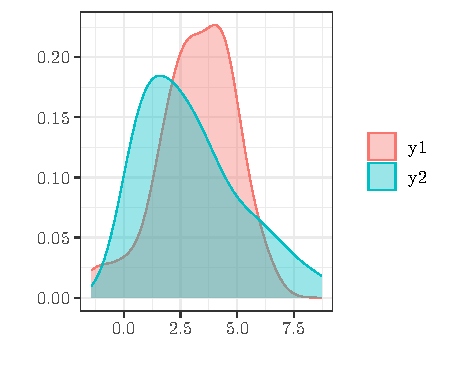
\includegraphics[width=\maxwidth]{figure/example-1} 

}

\caption[Simulated example]{Simulated example.}\label{fig:example}
\end{figure}

\end{knitrout}

Given that $p = .007$ we can conclude that there is a statistically significant difference between the two distributions. This result suggests that the overlapping method has detected differences that the previous $t$-tests did not identify, highlighting the potential sensitivity of this approach.


\section{Simulation study}

To evaluate the performance of the permutation test applied to the overlapping index, we performed a simulation study. The aim is to generate data for a set of scenarios distinguishing mean, variance and shape of the populations and compare the $\zeta$ perm test to other commonly used tests in terms of type I error control and power. 

\subsection{Data generation}

In the simulation, two density distributions will be compared for many different scenarios. The first distribution will always be a normal standard distribution with $\mu = 0$ and $\sigma = 1$. 
To simulate data for the second distribution we use the Skew-Normal distribution \cite{azzalini:1985}, which is defined in the following way: given $\xi \in \mathbb{R}$, $\omega \in \mathbb{R}^{+}$ and $\alpha \in \mathbb{R}$, then for $y \in \mathbb{R}$ we have  
\begin{equation}
\resizebox{\columnwidth}{!}{$
\mathcal{SN}(y|\xi, \omega, \alpha) = \frac{1}{\omega \sqrt{2\pi}} \exp \left[ -\frac{1}{2} \left( \frac{y-\xi}{\omega} \right)^2  \right] \left[ 1+ \text{erf}\left( \alpha \left( \frac{y-\xi}{\omega\sqrt{2}}\right) \right) \right]
$}
\end{equation}
in which $$\text{erf}(z) = \frac{2}{\sqrt{\pi}} \int_{0}^{z} e^{-t^2} dt $$ is the \emph{error function}.
When $\xi = 0$, $\omega = 1$ and $\alpha = 0$ the distribution is a standard normal distribution.

$\xi$ is the location parameter, $\omega$ is the scale parameter and $\alpha$ is related to the skewness of the distribution. Therefore, this distribution is suitable to generate data modelling both the distance between means (the effect size), symmetry and variance.


\begin{figure*}[!h]
\begin{knitrout}
\definecolor{shadecolor}{rgb}{0.969, 0.969, 0.969}\color{fgcolor}

{\centering 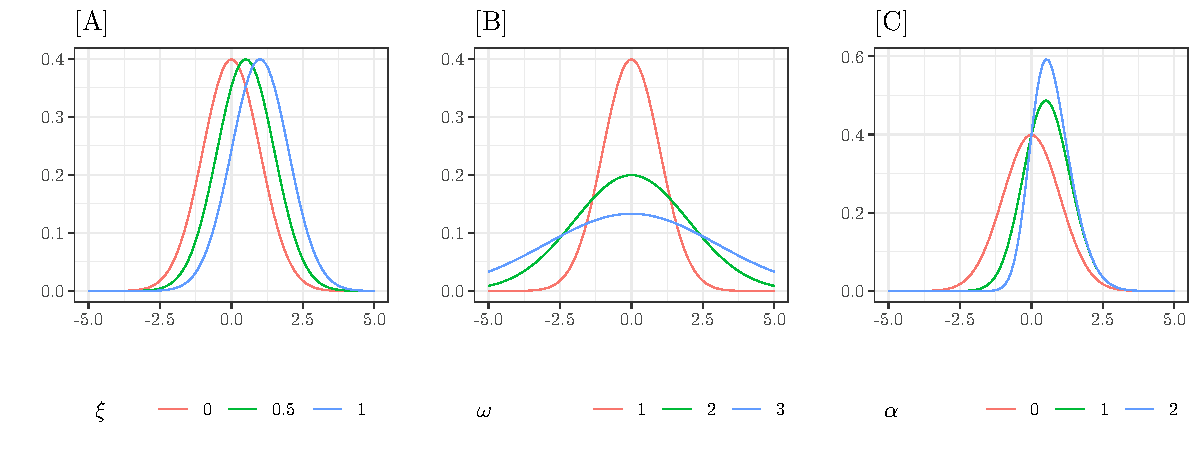
\includegraphics[width=\maxwidth]{figure/scenari-1} 

}


\end{knitrout}
\caption{Examples of Skew-Normal distributions ($\xi$,$\omega$,$\alpha$); [A] three densities with same variance and shape but different location parameter values ($\xi = 0, 0.5, 1$), [B] three densities with same mean and shape but different scale parameter values ($\omega = 1, 2, 3$) and [C] three densities with same mean and variance but different shape parameter values ($\alpha = 0, 1, 2$). \label{fig:scenari}}
\end{figure*}

Mean and variance of the Skew-Normal are respectively: 
\begin{eqnarray}\label{eq:musigmaSN}
\begin{array}{l}
\mu = \xi + \omega \gamma \sqrt{2/\pi} \\
\sigma^2 = \omega^2 [1- (2\gamma^2)/\pi]
\end{array}
\end{eqnarray}
in which $\gamma = \alpha / \sqrt{1 + \alpha^2}$. Based on the equations (\ref{eq:musigmaSN}) we can determine the values to assign to the parameters $\xi$ e $\omega$ in function of $\mu$ and $\sigma$ with the equations:

\begin{eqnarray}\label{eq:xiomegaSN}
\begin{array}{l}
 \xi = \mu - \omega \gamma \sqrt{2/\pi} \\
 \omega = \sqrt{\sigma^2/ [1- (2\gamma^2)/\pi]}
\end{array}
\end{eqnarray}

The Skew-Normal distribution is optimal for our purpose as it allows to have control over parameters of mean, variance, skewness and kurtosis, as shown in figure \ref{fig:scenari}.

\subsection{Simulation design}




In the simulation we confront two samples extracted from a Skew-Normal, the first one is generated from $\mathcal{SN}(0,1,0)$, which is the Standard-Normal distribution, and the second one from $\mathcal{SN}(\xi,\omega,\alpha)$. Consequently, the first sample derives always from a population with mean 0 and variance 1. To define the various scenarios, we manipulate the parameters of the second population in orther to obtain specific differences in means ($\delta$), standard deviations ($\sigma$) and skewness ($\alpha$). Four factors were sistematically varied ina complete four-factors design as follows:

\begin{itemize}

   \item $\delta = (0, 0.2, 0.5, 0.8)$; mean of the second population, which corresponds also to the difference between the two groups, the first one has always $\mu = 0$;
  \item $\sigma = (1, 2, 3)$; standard deviation of the second population;
  \item $\alpha = (0, 2, 10)$; degree of asymmetry (skewness) of the second population; 
  \item $n = (10, 20, 50, 100, 500)$; sample size, equal in the two samples.
 
  %\item N simulation: NTAB[1,1,1,1] for each combination of parameters

\end{itemize}


For each of the $4 \times 3 \times 3 \times 5 = 180$ conditions we generated 3000 sets of data on which we performed the analysis. 








\begin{figure*}
%,fig.width=7,fig.cap=" ",fig.height=9
\begin{knitrout}
\definecolor{shadecolor}{rgb}{0.969, 0.969, 0.969}\color{fgcolor}

{\centering 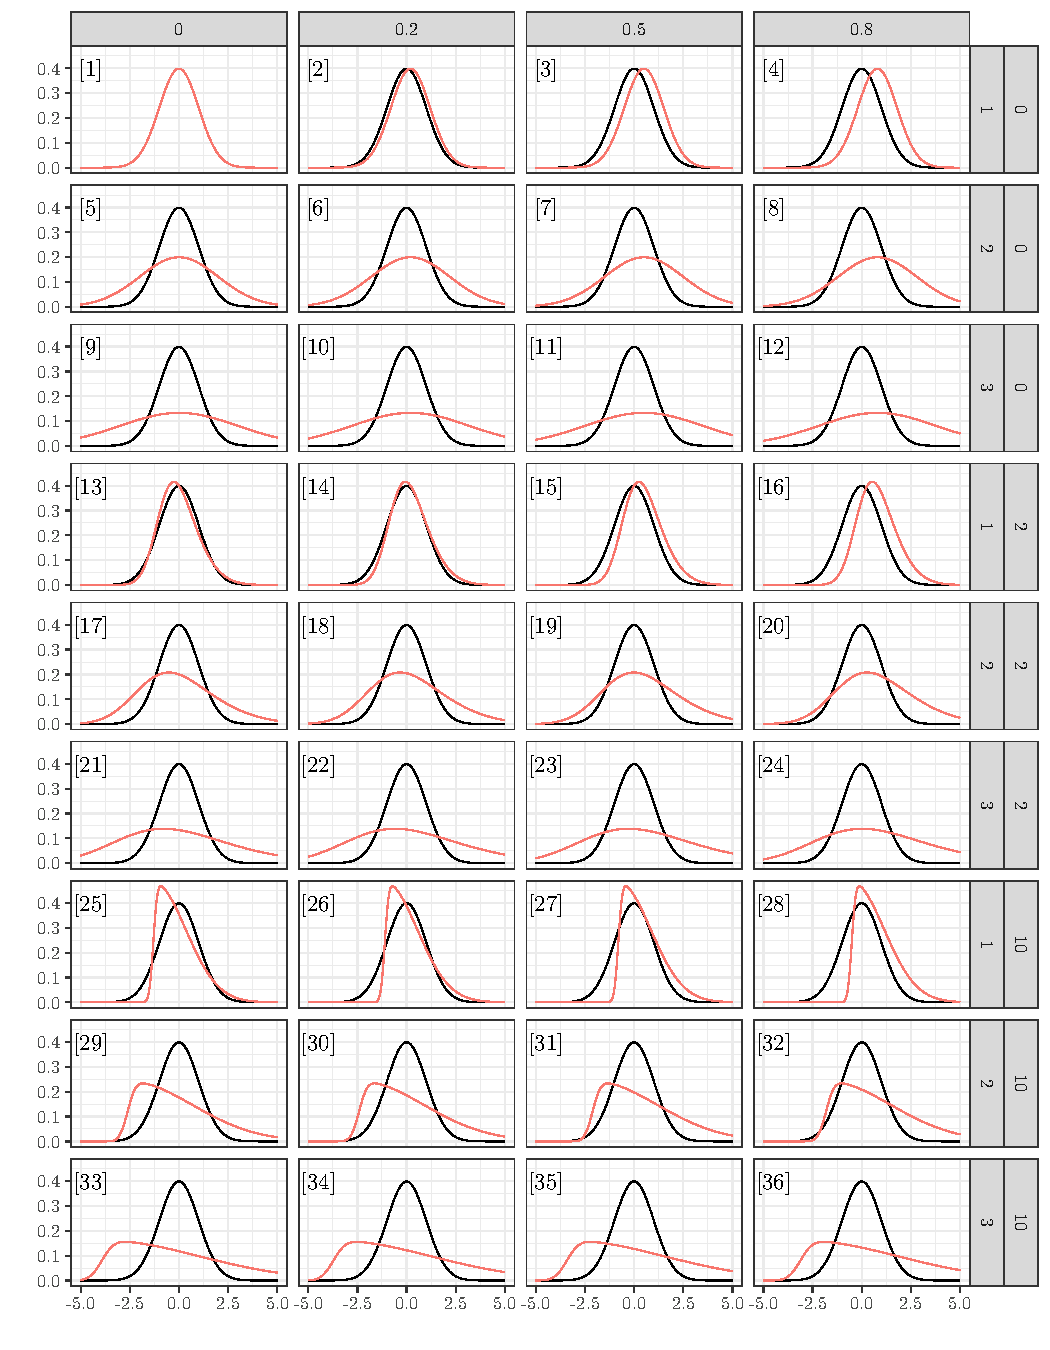
\includegraphics[width=\maxwidth]{figure/alpha0-1} 

}


\end{knitrout}
\caption{Generative data distributions in function of $\delta$ (column panels) and $\sigma$ (row panels). The black curves are the first sample, $\mathcal{SN}(0,1,0)$, the red ones represent second sample.\label{fig:alpha0}}
\end{figure*}

In figure \ref{fig:alpha0} are graphically represented the 36 scenarios of data generation, the black curves are the first population, always a $\mathcal{SN}(0,1,0)$, and the red curves are relative to the second population $\mathcal{SN}(\xi,\omega,\alpha)$.

For each combination $\delta \times \sigma \times \alpha \times n $, on the generated data were performed the following tests: 
\begin{itemize}
 \item $t$ test for independent samples, assuming equal variance;
 \item Welch test for independent samples;
 \item Wilcoxon test for independent samples;
 \item Permutation test on the complement of the overlapping index, $\zeta = 1-\eta$, which therefore becomes an index of difference between groups;
 \item $F$ test of homogeneity of variances;
 \item Kolmogorov-Smirnov test for comparing two distributions.
\end{itemize}

The whole procedure generated a total of 540000 datasets as well as 3240000 of statistical tests and corresponding $p$-values.

% \begin{itemize}
%  \item T-test: a parametric test used to test if the mean value of a distribution is significantly different from the one of another group;
%  \item Welch test: as a variation of the independent sample t-test, this one does not assume equal variance between the two groups, and is therefore more robust when variance or sample size is different in the two groups;
%  \item Wilcoxon Signed-Rank Test: is a non parametric test to compare two related samples or a single repeated measure on the same sample when the data is not normally distributed and is based on the mean rank difference;
%  \item Variance test (F-test): a parametric test to compare the variance in two groups or more. It relies on normality assumptions and the null hypotesis is equal variance in the two groups;
%  \item Kolmogorov-Smirnov Test: a non-parametric test used to either compare a sample distribution to a known distribution or to compare two samples to test if they come from the same unknown distribution;
%  \item T-test with permutation approach: is a test on means but the p-value is calculated through permutations, therefore it is not parametric;
%  \item F-test with permutation approach: is a test on variance and again, it is a non parametric test calculating the p-value through permutations of the data;
%  \item Overlapping index $\zeta$ with permutation approach.
% \end{itemize}


\subsection{Definition of Statistical tests}

We introduce the chosen statistical tests summarizing the specific hypothesis and assumptions for each one. 

\subsubsection{$t$ test}

This is the classic case of a test for independent samples assuming equal variances and the normality of the two distributions:
 
\begin{eqnarray*}
H_0: \mu_1 - \mu_2 = 0 \mbox{ with } \sigma_1 = \sigma_2
\end{eqnarray*}

% Therefore, in the scenarios from which the samples come from populations with same mean -- figure \ref{fig:alpha0}, panels in the first left column, [1, 5, 9, 13, 17, 21, 25, 29, 33] -- type I error control is estimated, meanwhile, power is estimated for the remaining scenarios. Note that assumption of homogeneity of variance for this test are met only in the scenarios in the first row.

\subsubsection{Welch (W) test}

This is the $t$ test modified when homogeneity of variances is not respected:

\begin{eqnarray*}
H_0: \mu_1 - \mu_2 = 0 \mbox{ with } \sigma_1 \neq \sigma_2
\end{eqnarray*}

Also this test assumes the normality.

%Control of type I error is estimated for the same scenarios as for the $t$ test, as well as for the power.

\subsubsection{Wilcoxon-Mann-Whitney (WMW) test}

This is the test on ranks which evaluates the following hypothesis without assumptions on distributions:
 
\begin{eqnarray*}
H_0: P(X_1 > X_2) = P(X_2 > X_1) = 0.5
\end{eqnarray*} 

in which $X_1$ and $X_2$ are the random variables representing the observations extracted from the two populations. %In this case, the only scenario in which $H_0$ is true is in panel [1]. Given that this is a distribution free test, assumptions are not required.

\subsubsection{Kolmogorov-Smirnov (KS) test}

This test compares the cumulative distributions $$H_0: F(X_1) = F(X_2)$$ without assumptions on distributions. %the null hypothesis should be true in panel [1], as it is for the  $\zeta$  permutation test.

\subsubsection{$F$ test}

This is the test of homogeneity of variances $$H_0: \sigma^2_1 = \sigma^2_2$$ assuming the normality. %the condition is true in all scenarios where $\sigma = 1$, panels [1-4, 13-16, 25-28]. In those scenarios we estimate type I error, in all the others we calculate power.

\subsubsection{ $\zeta$  overlapping ($\zeta_{\mbox{ov}}$) test}

Since $\zeta = 1 - \eta$, in which $\eta$ is the area of overlapping of the empirical distributions, the null hypothesis of the test is $$H_0: \zeta = 0$$ which implies that the data comes from the same population, or from populations with same shape (mean, variance and skewness) but without specific assumptions. %Therefore, the only condition in which $H_0$ is true is the first panel, [1]. Also in this case, the test does not require particular assumptions.

%\vspace{.3cm}

\section{Results}

First of all, we analysed correlations between the $p$-values of the considered tests in order to assess how much they are associated independently from the experimental condition.

Next, we considered panel [1], figure \ref{fig:alpha0}, the scenario in which all null hypothesis are true and assumptions are respected for all tests. Consequently, we computed type I error by counting how many times the test is significant in this scenario, and the power by counting how many times it will be significant in all other scenarios. In this way, we evaluated type I error and power based on the experimental conditions.

%Then we will consider separately the cases in which assumptions are respected and when they are not.

\subsection{Correlations among tests}

Figure \ref{fig:correlazioni} represents the correlation matrix between the $p$-values for the different tests in all experimental conditions. The classical tests show an order in the way they correlate. More specifically, $t$ and W tests show a perfect correlation, WMW is highly correlated with the aforesaid tests, and the KS shows a lower but still medium-large correlation. $F$ presents no correlation with $t$, W and WMW tests, and medium correlation with the $\zeta_{\mbox{ov}}$ and KS tests. 

The $\zeta_{\mbox{ov}}$ test is highly correlated with the KS test, has a lower correlation with tests on means ($t$ and W) and ranks (WMW), and a medium correlation with the $F$ test.



%% ,fig.width=5,fig.height=4
\begin{knitrout}
\definecolor{shadecolor}{rgb}{0.969, 0.969, 0.969}\color{fgcolor}\begin{figure}[!t]

{\centering 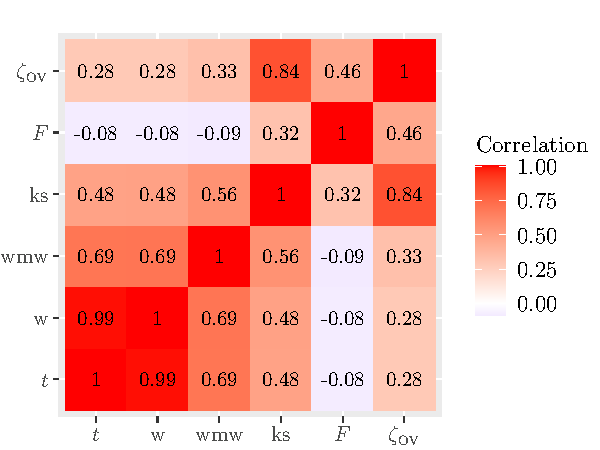
\includegraphics[width=\maxwidth]{figure/correlazioni-1} 

}

\caption[Correlation matrix among $p$-values $(N = 540000)$ in chosen tests]{Correlation matrix among $p$-values $(N = 540000)$ in chosen tests. Note: ks = Kolmogorov-Smirnov test, $\zeta_{\mbox{ov}}$ = $\zeta$  overlapping test, $F$ = variance test, wilcoxon = Wicoxon-Mann-Whitney test, welch = Welch test, $t$ = Student's $t$ test.}\label{fig:correlazioni}
\end{figure}

\end{knitrout}




\subsection{Type I error and power}





In figure \ref{fig:global}, is represented type I error in panel [A] and power in panel [B] estimated considering as true null hypothesis the situation in which samples are drawn from two exactly equal populations (figure \ref{fig:alpha0}, panel [1]).

In relation to type I error, all tests show a good performance, whereas the KS test is too conservative for small samples. 

Concerning power, the $\zeta$ overlapping test outperforms all other tests, already with small sample sizes. From the graphical representation it is visible how two subgroups can be identified: one including the tests on means and ranks, not reaching adequate power even with large samples, and the second one formed by the $\zeta_{\mbox{ov}}$ and KS tests, reaching good power already from 100 observations, with the $\zeta_{\mbox{ov}}$ outperforming the KS test reaching good power already from 50 observations.

%as different tests have different null hypothesis. 

%,fig.cap="",
\begin{figure*}[!h]
\begin{knitrout}
\definecolor{shadecolor}{rgb}{0.969, 0.969, 0.969}\color{fgcolor}

{\centering 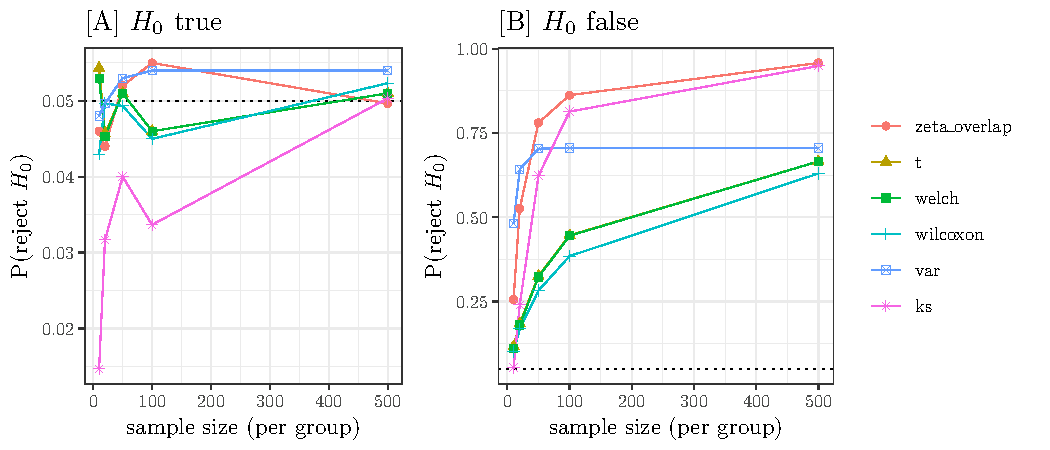
\includegraphics[width=\maxwidth]{figure/global-1} 

}


\end{knitrout}
\caption{Control of type I error [A] and power [B] in the various tests.\label{fig:global}}
\end{figure*}



\section{Discussion}

% The high correlation between the \textbf{$t$-test} and \textbf{Welch test} reflects their similar objectives, particularly in testing mean differences. However, the lower correlations between parametric and non-parametric tests, such as the \textbf{Wilcoxon} and \textbf{KS} tests, indicate that these tests capture different aspects of the data (e.g., ranks or distribution shapes rather than means). The $F$-test is not related to parametric and \textbf{Wilcoxon} tests, given that it evaluates variance, whereas in the other tests the focus is on different aspects. The said test however shows medium to large correlations with the \textbf{KS} and $\zeta_{\mbox{ov}}$
% 
% The \textbf{permutation-based tests} is highly correlated with the \textbf{KS} tests, as they are most similar in considering the distribution, rather than specific parameters. Moreover, in relation to the remaining tests it shows medium correlations, indicating how they are similar 
% 
% exhibit intermediate correlations with both parametric and non-parametric methods, indicating that their results may align with both types depending on the underlying data structure.

The analysis of $p$-value correlations among the tests provides insight into their relationships. High correlation between the $t$-test and W test, for instance, reflects their similar objectives and shared focus on mean differences. However, lower correlations between parametric and non-parametric methods, such as the WMW and KS tests, indicate that these tests capture distinct aspects of the data, such as ranks or distribution shapes rather than means. The permutation-based tests show intermediate correlations with both parametric and non-parametric methods, which suggests that they may align with either types of tests depending on the underlying data structure, highlighting the versatility of the $\zeta_{\mbox{ov}}$ test.


Moreover, the present analysis evaluated the performance of various statistical significance tests across simulated scenarios comparing each test on the same null hypothesis, being no difference in the two populations from which the samples are drawn. The tests include both parametric (such as the T-test, Welch test, and F-test for variance) and non-parametric methods (such as the Wilcoxon Signed-Rank, Kolmogorov-Smirnov, and permutation-based approaches including the $\zeta_{\mbox{ov}}$ test). Through these scenarios, we assess each test's robustness, Type I error control, and power.

In figure \ref{fig:global}, panel [A], the only test which is over-conservative in terms of Type I error is the $F$ test, yet reaching the nominal $0.05$ level with bigger samples (over 400 observations). All other tests, already from small samples, are in the range of $0.045 - 0.055$, converging closer to $0.05$ as sample size grows, except for the $F$ test remaining less conservative than the others. From this analysis we can then conclude that all tests are able to control Type I error for bigger samples, yet caution is needed for small samples when using the $F$ test.

Concerning power, panel [B], the $\zeta_{\mbox{ov}}$ test outperforms all other tests. The only one competing with good power is the KS test, reaching a power of 60\% with 50 observations and aligning with the $\zeta_{\mbox{ov}}$ at 500 observations. The $F$ test starts at higher power for small samples but fails to reach an adequate power of 80\%. W and $t$ tests performances are identical, in line with their perfect correlation of $p$-values, never exceeding 60\% of power and performing consistently worse than the $\zeta_{\mbox{ov}}$ and KS tests, especially with small samples. Lastly, the WMW test performs similarly to $t$ and W tests with slightly less power throughout the increase of sample size. These results highlight the outstanding performance of the $\zeta_{\mbox{ov}}$ test already from small samples, showing an advantage in choosing this test in research settings regardless of data distribution and assumptions.

\subsection*{Advantages and Limitations of the $\zeta$ Permutation Test}

The \textbf{$\zeta$  overlapping test}, designed to measure the degree of overlap between distributions, has specific advantages and limitations. Its main strength lies in its robustness to distributional assumptions, as it calculates p-values through permutations rather than relying on parametric assumptions like normality or equal variance. This makes it particularly useful in scenarios where other tests may fail due to assumption violations, providing a conservative Type I error rate when \(H_0\) is true and robust power when \(H_0\) is false.

The main limitation of the test is that it does not inform on specific parametric differences, as its design focuses on distributional overlap rather than mean differences, which means it does not directly inform on mean, variance or skewness differences specifically. But we argue that the $\zeta_{\mbox{ov}}$ test offers a great starting point to evaluate whether two distributions differ in the first place with high power already from small samples. Moreover, the package to compute the index also offers the possibility to plot densities and the area of overlap, therefore making it extremely intuitive to visualize how the two distributions practically differ. In cases in which the test fails to find a difference between the two distributions one can conclude that the two groups/conditions do not differ in any parameter of possible interest, but if the test finds a statistically significant difference, then the researcher can move on to test which are the specific parameters differring between the two. This approach highlights the importance of visualizing data and stresses out the invalue insight offered by descriptive statistics.

The $\zeta$ permutation test is indeed a valuable tool for non-parametric inference, particularly when distributional assumptions do not meet those required by common statistical test e.g. $t$-test. These are particularly relevant points given that in psychological sciences studies often involve small sample sizes, and relying on small changes in location parameters like the mean can be risky. For example, small samples are highly susceptible to the influence of extreme values, which can skew the mean and lead to misleading conclusions about effect sizes. Even more importantly, as demonstrated in simulations, the $\zeta_{\mbox{ov}}$ test is less prone to being dramatically impacted by extreme values, as it directly measures the distributional overlap between groups rather than focusing solely on mean differences. This characteristic makes such test particularly valuable in small-sample contexts, especially in psychological science where robustness to outliers is critical for obtaining reliable insights into group differences.

\section{Conclusion}

By exploring alternative scenarios, the study offers practical indication to operate a shift in the philosophical approach to data analysis and significance testing. In fact, the Overlapping index forces the functional interpretation of the results to move beyond significance testing alone \cite{pastore2018overlapping, steegen2016increasing, gelman2018failure}. In psychological research, considering the distribution of data rather than relying solely on significance testing offers a deeper, more nuanced understanding of results. Traditional significance testing doesn't provide information about the nature or magnitude of that effect. By visualizing and considering the entire distribution of data, researchers can observe the spread, central tendency, and shape of the data, which often reveal valuable insight about variability and individual differences within the sample.  As presented in figure \ref{fig:example}, reporting a mean difference without an understanding of the data's variability could lead to misrepresentation of the consistency or generalizability of the observed effect. Therefore, incorporating distributional analyses allows psychologists to present a fuller picture of their findings, improving both interpretability and transparency in their research conclusions. 

Moreover, the present study further underscores the necessity of reasoning on the most suitable statistical tools contingent on the specific characteristics of the data and the assumptions inherent in the analytical techniques employed. Such a switch in the philosophical approach to data analysis in psychological sciences \cite{vasishth2021embrace} may improve the robustness and validity of psychological research findings, allowing for more aware interpretations and generalizations. We stress this by making open available data and material so that such an approach might be useful for a wide range of psychologists interested in increasing the understandability of their results. 

The findings underscore the necessity of choosing statistical methods that are resilient to the complexities inherent in psychological data, where assumption violations are often inevitable. The $\zeta$ overlapping test is a robust alternative to commonly used tests in psychological science that accommodates data with unequal variances or non-normal distributions, offering reliable results even when classic parametric conditions are unmet. In this way, our test extends the flexibility of significance testing, enabling a nuanced understanding of effects in psychology.

Ultimately, statistics in psychology should reflect both theoretical knowledge and an appreciation for the distributional nuances of psychological variables. Rather than a rigid application of conventional methods, statistical analysis should be a deliberate choice that aligns with the nature of the data and the research question. The approach of the $\zeta$ overlapping test embodies this principle, capturing the depth and complexity of psychological effects in a way that is both methodologically rigorous and sensitive to the real-world structure of psychological phenomena.

\subsection*{Legenda}

$\eta$ is the area of overlap

\noindent $\zeta$ is the area of non overlap, therefore $1 - \eta$

\noindent $\mu$ is the parameter of the mean of the normal standard 

\noindent $\sigma$ is the standard deviation of the normal standard

\noindent $\delta$ is the difference between the two means

\noindent $\xi$ is the location parameter of the skew-normal

\noindent $\omega$ is the scale parameter of the skew-normal

\noindent $\alpha$ determins the simmetry of the skew-normal


\subsection*{Ethical considerations}
Ethical approval was not required

\subsection*{Conflicting interest}
The authors declare no conflict of interests.

\subsection*{Funding statement}
No Funding supported this project.

\bibliographystyle{apacite}
\bibliography{overlap}
\end{document}

\section{Data availability statement}
Data and materials to reproduce the present work are openly available at \href{https://github.com/ambraperugini/Overlapping}{GitHub} 


\bibliographystyle{apacite}
\bibliography{overlap}

\end{document}


%%%%%%%%%%%%%%%%%%%%%%%%%%%%
\section{FINO QUI}
\bibliographystyle{apacite}
\bibliography{overlap}

\end{document}
%%%%%%%%%%%%%%%%%%%%%%%%%%%%



%%%%%%%%%%%%%%%%%%%%%%%%%%%%%%%
\subsection{Assumptions and type I error and power}

In the top row of figure \ref{fig:assunzioni} are represented type I error and power for cases in which assumptions are respected. The patter is similar to the scenario in \ref{fig:global} where there was no distinction for the assumptions, confirming the good control of type I error of the $\zeta$ perm test and greater power of the test in comparison to the others.
As not all tests that we performed imply assumptions, we only computed type I error and power for those tests that can have the assumptions violated ($t$ test, $F$ test, Welch test). What emerges is a bad control of type I error of the $F$ test.




\begin{knitrout}
\definecolor{shadecolor}{rgb}{0.969, 0.969, 0.969}\color{fgcolor}\begin{figure}[!b]

{\centering 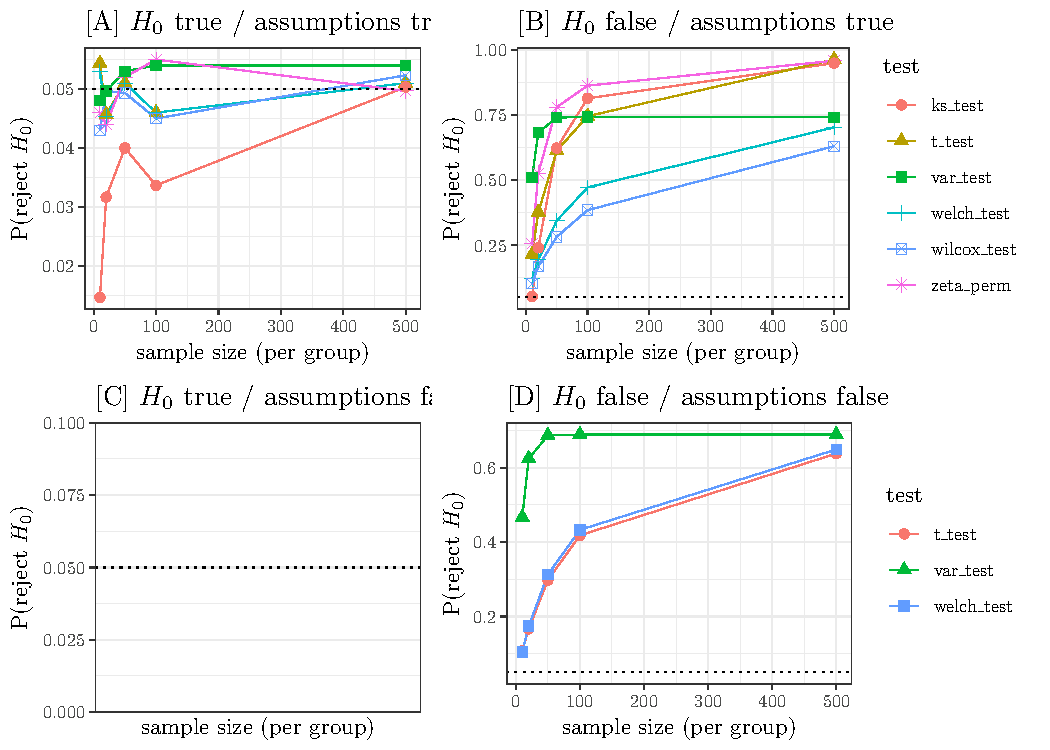
\includegraphics[width=\maxwidth]{figure/assunzioni-1} 

}

\caption[Control of type I error and power for scenarios in which assumptions are respected (top panels) and when they are not (bottom panels)]{Control of type I error and power for scenarios in which assumptions are respected (top panels) and when they are not (bottom panels).}\label{fig:assunzioni}
\end{figure}

\end{knitrout}



%%\subsection{gara tra $\zeta$ perm da solo e t-test, ks e var test }
\section*{Comparison of Statistical Tests Across Simulated Scenarios}

In this analysis, we compared the performance of several statistical significance tests across different simulated scenarios starting from a real data collection, where assumptions were either met or violated, and the null hypothesis (\(H_0\)) was either true or false. The simulation study starting from the real dataset emerged to be an informative approach that allowed to evaluate the significance testing performance across statistical test knowing the \textit{ground truth} beyond the data generation. The tests evaluated include both parametric (e.g., T-test, Welch test, F-test for variance) and non-parametric tests (e.g., Wilcoxon Signed-Rank, Kolmogorov-Smirnov, and permutation-based tests, including $\zeta$ permutation). Each scenario provides insight into the robustness, power, and Type I error control of these methods under varied conditions. 


\subsection*{Scenario A: \(H_0\) True, Assumptions Met}

In Scenario A, where \(H_0\) is true and the assumptions are satisfied, all tests ideally should maintain Type I error close to the nominal level of 0.05. Here, we observe that:

\begin{itemize}
    \item The \textbf{T-test} and \textbf{Welch test} control Type I error well, as expected for parametric tests under ideal conditions. The Welch test shows slightly more variability in Type I error, likely due to its adjustment for unequal variances, though this remains within an acceptable range.
    \item The \textbf{Wilcoxon Signed-Rank test} and the \textbf{Kolmogorov-Smirnov (KS) test} appear slightly conservative, producing Type I error rates below the nominal level. This conservative behavior is typical of non-parametric tests that are more robust to non-normality, though they may reduce sensitivity when assumptions are fully met.
    \item The \textbf{ $\zeta$  permutation test} is also conservative, which could indicate its suitability for controlling Type I error in scenarios where overlap between distributions is the focus. 
    \item The \textbf{permutation-based T-test} and \textbf{F-test} yield Type I error rates close to the nominal level, benefiting from the flexibility of permutation-based p-value calculation even when assumptions are met.
\end{itemize}

In summary, under ideal conditions, most tests perform as expected, with parametric tests aligning closely with the nominal Type I error and non-parametric and permutation methods showing slight conservatism.



\subsection*{Scenario B: \(H_0\) False, Assumptions Met}

When \(H_0\) is false and assumptions are met (Scenario B), power is the primary metric of interest. Here, we find:

\begin{itemize}
    \item The \textbf{Welch test} demonstrates high power, surpassing the T-test as sample size increases, due to its flexibility with unequal variances. This makes it a robust choice when variances may differ even if assumptions of normality are met.
    \item The \textbf{permutation-based T-test} and \textbf{ $\zeta$  permutation test} also exhibit high power, highlighting their effectiveness in detecting true effects without relying on strict distributional assumptions.
    \item Non-parametric tests, such as the \textbf{Wilcoxon} and \textbf{KS} tests, show moderate power, though they are generally less sensitive to mean differences than parametric alternatives. Their focus on distribution shapes or ranks limits their power when mean differences are the primary effect.
\end{itemize}

In this scenario, the Welch test and permutation-based methods emerge as highly effective for detecting differences, especially when variances may differ, while non-parametric tests are somewhat limited in sensitivity.

\subsection*{Scenario C: \(H_0\) True, Assumptions Violated}

When assumptions are violated but \(H_0\) remains true (Scenario C), Type I error control becomes crucial. This scenario reveals the robustness of each test under non-ideal conditions:

\begin{itemize}
    \item The \textbf{Welch test} maintains Type I error control effectively, showcasing its robustness to heteroscedasticity and other violations. This highlights its utility in practical scenarios where equal variance cannot be guaranteed.
    \item The \textbf{permutation-based tests} (both for means and variances) also perform well, maintaining Type I error near the nominal level, thanks to their non-parametric approach to p-value calculation. 
    \item The \textbf{T-test} and \textbf{Variance (F) test} exhibit increased sensitivity to assumption violations, particularly the F-test, which shows inflated Type I error rates under heteroscedasticity and non-normality. This sensitivity reduces their reliability in practical applications where assumptions are not met.
    \item Non-parametric tests, like the \textbf{Wilcoxon} and \textbf{KS tests}, handle assumption violations effectively, producing conservative Type I error rates. Their robustness to non-normality makes them a safer choice when parametric assumptions are doubtful.
\end{itemize}

Under assumption violations with a true null hypothesis, the Welch and permutation-based tests stand out as reliable choices, while the F-test is notably sensitive to violations.

\subsection*{Scenario D: \(H_0\) False, Assumptions Violated}

In the final scenario, where both \(H_0\) is false and assumptions are violated (Scenario D), the adaptability of each test is evaluated under the most challenging conditions:

\begin{itemize}
    \item The \textbf{Welch test} maintains high power, adapting well to heteroscedasticity and other assumption violations. This underscores its suitability for real-world data where variances may be unequal and normality cannot be assumed.
    \item The \textbf{permutation-based T-test} and \textbf{ $\zeta$  permutation test} also demonstrate strong performance, showing that permutation-based approaches can be powerful alternatives when assumptions do not hold.
    \item Non-parametric tests like \textbf{Wilcoxon} and \textbf{KS} show moderate power but generally lag behind parametric tests in detecting mean differences. They remain robust to assumption violations but are less efficient in detecting differences in means, particularly with skewed distributions.
    \item The \textbf{Variance (F) test} performs poorly in this scenario, with both reduced power and increased error rates, underscoring its sensitivity to assumption violations. Its reliance on equal variance assumptions makes it unsuitable in situations where homoscedasticity cannot be assured.
\end{itemize}

In this scenario, the Welch test and permutation methods again emerge as the most adaptable, providing good power even when assumptions are substantially violated.
